%\documentclass{beamer}
\documentclass[aspectratio=169]{beamer}


%
% Choose how your presentation looks.
%
% For more themes, color themes and font themes, see:
% http://deic.uab.es/~iblanes/beamer_gallery/index_by_theme.html
%
\mode<presentation>{
  \usetheme{Madrid}      % or try Darmstadt, Madrid, Warsaw, AnnArbor
  \usecolortheme{wolverine} % or try albatross, beaver, crane, ... deafult, wolverine
  \usefonttheme{default}  % or try serif, structurebold, ...
  \setbeamertemplate{navigation symbols}{}
  \setbeamertemplate{caption}[numbered]
}
\usepackage[english]{babel}
% \usepackage[T2A]{fontenc}
\usepackage[utf8x]{inputenc}
\usepackage{quiver}
\usepackage{amssymb,amsmath,amsthm}
%\usepackage{algorithm}
%\usepackage{algpseudocode}

%-------------------------------------------------

%\def\hidentxt#1{{#1}}
\def\hidentxt#1{\uncover<+->{#1}}
%-------------------------------------------------
\def\thm#1{\begin{block}{Definition}
#1
\end{block}}


%%%%%%%%%%%%%%%%%%%%%%%%%%%%%%%%%%%%%%%%%%%%%%%%%%%%%%%%%%%%%%%%%%%%%%%%%%%%
\title[Graph Isomorphism]{A Graph Isomorphism Algorithm}
\date{\today}
\author[G. Woodworth]{Glen Woodworth}
\institute[UAF]{
   Department of Mathematics and Statistics%
   \\%
   University of Alaska Fairbanks%
}

\begin{document}

\begin{frame}
  \titlepage
\end{frame}

\begin{frame}{Graphs}

    \thm{An undirected, simple graph $G=\{V,E\}$ is a set of vertices $V$, and a set of edges, $E$,  where $E$ is a set of unordered pairs of vertices from $V$ such that for all $u\in V$, $\{u,u\}\notin E$.  }
   % https://q.uiver.app/?q=WzAsMTUsWzMsMSwiXFxidWxsZXQiXSxbNCwyLCJcXGJ1bGxldCJdLFs0LDEsIlxcYnVsbGV0Il0sWzMsMiwiXFxidWxsZXQiXSxbNSwxLCJcXGJ1bGxldCJdLFs2LDAsIlxcYnVsbGV0Il0sWzcsMSwiXFxidWxsZXQiXSxbNywyLCJcXGJ1bGxldCJdLFs2LDMsIlxcYnVsbGV0Il0sWzUsMiwiXFxidWxsZXQiXSxbMCwxLCJcXGJ1bGxldCJdLFswLDIsIlxcYnVsbGV0Il0sWzEsMiwiXFxidWxsZXQiXSxbMiwyLCJcXGJ1bGxldCJdLFsxLDEsIlxcYnVsbGV0Il0sWzAsMSwiIiwyLHsic3R5bGUiOnsiaGVhZCI6eyJuYW1lIjoibm9uZSJ9fX1dLFsxLDIsIiIsMix7InN0eWxlIjp7ImhlYWQiOnsibmFtZSI6Im5vbmUifX19XSxbMiwzLCIiLDIseyJzdHlsZSI6eyJoZWFkIjp7Im5hbWUiOiJub25lIn19fV0sWzQsNSwiIiwyLHsic3R5bGUiOnsiaGVhZCI6eyJuYW1lIjoibm9uZSJ9fX1dLFs1LDYsIiIsMix7InN0eWxlIjp7ImhlYWQiOnsibmFtZSI6Im5vbmUifX19XSxbNiw3LCIiLDIseyJzdHlsZSI6eyJoZWFkIjp7Im5hbWUiOiJub25lIn19fV0sWzcsOCwiIiwyLHsic3R5bGUiOnsiaGVhZCI6eyJuYW1lIjoibm9uZSJ9fX1dLFs4LDksIiIsMix7InN0eWxlIjp7ImhlYWQiOnsibmFtZSI6Im5vbmUifX19XSxbOSw0LCIiLDIseyJzdHlsZSI6eyJoZWFkIjp7Im5hbWUiOiJub25lIn19fV0sWzEwLDExLCIiLDAseyJzdHlsZSI6eyJoZWFkIjp7Im5hbWUiOiJub25lIn19fV0sWzExLDEyLCIiLDAseyJzdHlsZSI6eyJoZWFkIjp7Im5hbWUiOiJub25lIn19fV0sWzEyLDEzLCIiLDAseyJzdHlsZSI6eyJoZWFkIjp7Im5hbWUiOiJub25lIn19fV0sWzExLDE0LCIiLDAseyJzdHlsZSI6eyJoZWFkIjp7Im5hbWUiOiJub25lIn19fV1d
\[\begin{tikzcd}[ampersand replacement=\&]
	\&\&\&\&\&\& \bullet \\
	\bullet \& \bullet \&\& \bullet \& \bullet \& \bullet \&\& \bullet \\
	\bullet \& \bullet \& \bullet \& \bullet \& \bullet \& \bullet \&\& \bullet \\
	\&\&\&\&\&\& \bullet
	\arrow[no head, from=2-4, to=3-5]
	\arrow[no head, from=3-5, to=2-5]
	\arrow[no head, from=2-5, to=3-4]
	\arrow[no head, from=2-6, to=1-7]
	\arrow[no head, from=1-7, to=2-8]
	\arrow[no head, from=2-8, to=3-8]
	\arrow[no head, from=3-8, to=4-7]
	\arrow[no head, from=4-7, to=3-6]
	\arrow[no head, from=3-6, to=2-6]
	\arrow[no head, from=2-1, to=3-1]
	\arrow[no head, from=3-1, to=3-2]
	\arrow[no head, from=3-2, to=3-3]
	\arrow[no head, from=3-1, to=2-2]
\end{tikzcd}\]
\end{frame}
% Uncomment these lines for an automatically generated outline.
%\begin{frame}{Outline}
%  \tableofcontents
%\end{frame}
%exampleblock -- green, alertblock -- red
\begin{frame}{Neighbors}
	\thm{
		For a graph $G=\{V,E\}$, if $\{u,v\}\in E$, we say $u$ and $v$ are \textit{adjacent} or \textit{neighbors}. The \textit{neighborhood} of $v\in G$, denoted $\mathcal{N}(v)$ is the set of all vertices $u\in G$ such that $v$ and $u$ are neighbors.}
% https://q.uiver.app/?q=WzAsMTgsWzMsMSwiXFxidWxsZXQiXSxbNCwyLCJcXGJ1bGxldCIsWzI3MCw2MCw2MCwxXV0sWzQsMSwidiIsWzI3MCw2MCw2MCwxXV0sWzMsMiwiXFxidWxsZXQiLFsyNzAsNjAsNjAsMV1dLFs1LDEsIlxcYnVsbGV0IixbMjQwLDYwLDYwLDFdXSxbNiwwLCJcXGJ1bGxldCJdLFs3LDEsIlxcYnVsbGV0Il0sWzcsMiwiXFxidWxsZXQiXSxbNiwzLCJcXGJ1bGxldCIsWzI0MCw2MCw2MCwxXV0sWzUsMiwicSIsWzI0MCw2MCw2MCwxXV0sWzAsMSwiXFxidWxsZXQiLFswLDYwLDYwLDFdXSxbMCwyLCJ1IixbMCw2MCw2MCwxXV0sWzEsMiwiXFxidWxsZXQiLFswLDYwLDYwLDFdXSxbMiwyLCJcXGJ1bGxldCJdLFsxLDEsIlxcYnVsbGV0IixbMCw2MCw2MCwxXV0sWzEsMywiXFxtYXRoY2Fse059KHUpIixbMCw2MCw2MCwxXV0sWzQsMywiXFxtYXRoY2Fse059KHYpIixbMjcwLDYwLDYwLDFdXSxbNywzLCJcXG1hdGhjYWx7Tn0ocSkiLFsyNDAsNjAsNjAsMV1dLFswLDEsIiIsMix7InN0eWxlIjp7ImhlYWQiOnsibmFtZSI6Im5vbmUifX19XSxbMSwyLCIiLDIseyJzdHlsZSI6eyJoZWFkIjp7Im5hbWUiOiJub25lIn19fV0sWzIsMywiIiwyLHsic3R5bGUiOnsiaGVhZCI6eyJuYW1lIjoibm9uZSJ9fX1dLFs0LDUsIiIsMix7InN0eWxlIjp7ImhlYWQiOnsibmFtZSI6Im5vbmUifX19XSxbNSw2LCIiLDIseyJzdHlsZSI6eyJoZWFkIjp7Im5hbWUiOiJub25lIn19fV0sWzYsNywiIiwyLHsic3R5bGUiOnsiaGVhZCI6eyJuYW1lIjoibm9uZSJ9fX1dLFs3LDgsIiIsMix7InN0eWxlIjp7ImhlYWQiOnsibmFtZSI6Im5vbmUifX19XSxbOCw5LCIiLDIseyJzdHlsZSI6eyJoZWFkIjp7Im5hbWUiOiJub25lIn19fV0sWzksNCwiIiwyLHsic3R5bGUiOnsiaGVhZCI6eyJuYW1lIjoibm9uZSJ9fX1dLFsxMCwxMSwiIiwwLHsic3R5bGUiOnsiaGVhZCI6eyJuYW1lIjoibm9uZSJ9fX1dLFsxMSwxMiwiIiwwLHsic3R5bGUiOnsiaGVhZCI6eyJuYW1lIjoibm9uZSJ9fX1dLFsxMiwxMywiIiwwLHsic3R5bGUiOnsiaGVhZCI6eyJuYW1lIjoibm9uZSJ9fX1dLFsxMSwxNCwiIiwwLHsic3R5bGUiOnsiaGVhZCI6eyJuYW1lIjoibm9uZSJ9fX1dXQ==
\[\begin{tikzcd}[ampersand replacement=\&]
	\&\&\&\&\&\& \bullet \\
	\textcolor{rgb,255:red,214;green,92;blue,92}{\bullet} \& \textcolor{rgb,255:red,214;green,92;blue,92}{\bullet} \&\& \bullet \& \textcolor{rgb,255:red,153;green,92;blue,214}{v} \& \textcolor{rgb,255:red,92;green,92;blue,214}{\bullet} \&\& \bullet \\
	\textcolor{rgb,255:red,214;green,92;blue,92}{u} \& \textcolor{rgb,255:red,214;green,92;blue,92}{\bullet} \& \bullet \& \textcolor{rgb,255:red,153;green,92;blue,214}{\bullet} \& \textcolor{rgb,255:red,153;green,92;blue,214}{\bullet} \& \textcolor{rgb,255:red,92;green,92;blue,214}{q} \&\& \bullet \\
	\& \textcolor{rgb,255:red,214;green,92;blue,92}{\mathcal{N}(u)} \&\&\& \textcolor{rgb,255:red,153;green,92;blue,214}{\mathcal{N}(v)} \&\& \textcolor{rgb,255:red,92;green,92;blue,214}{\bullet} \& \textcolor{rgb,255:red,92;green,92;blue,214}{\mathcal{N}(q)}
	\arrow[no head, from=2-4, to=3-5]
	\arrow[no head, from=3-5, to=2-5]
	\arrow[no head, from=2-5, to=3-4]
	\arrow[no head, from=2-6, to=1-7]
	\arrow[no head, from=1-7, to=2-8]
	\arrow[no head, from=2-8, to=3-8]
	\arrow[no head, from=3-8, to=4-7]
	\arrow[no head, from=4-7, to=3-6]
	\arrow[no head, from=3-6, to=2-6]
	\arrow[no head, from=2-1, to=3-1]
	\arrow[no head, from=3-1, to=3-2]
	\arrow[no head, from=3-2, to=3-3]
	\arrow[no head, from=3-1, to=2-2]
\end{tikzcd}\]
\end{frame}
\begin{frame}{Labelling}
	We want to talk about properties of specific vertices, so we give a label to each vertex. The vertices in the graphs below are labelled using the cardinality of their neighborhoods, also called the \textit{degree} of a vertex.
	
	% https://q.uiver.app/?q=WzAsMTUsWzMsMSwiMVxcYnVsbGV0Il0sWzQsMiwiXFxidWxsZXQgMiJdLFs0LDEsIlxcYnVsbGV0IDIiXSxbMywyLCIxXFxidWxsZXQiXSxbNSwxLCIyXFxidWxsZXQiXSxbNiwwLCJcXGJ1bGxldCAyIl0sWzcsMSwiXFxidWxsZXQgMiJdLFs3LDIsIlxcYnVsbGV0IDIiXSxbNiwzLCJcXGJ1bGxldCAyIl0sWzUsMiwiMlxcYnVsbGV0Il0sWzAsMSwiMVxcYnVsbGV0Il0sWzAsMiwiM1xcYnVsbGV0Il0sWzEsMiwiXFxidWxsZXQgMiJdLFsyLDIsIlxcYnVsbGV0IDEiXSxbMSwxLCJcXGJ1bGxldCAxIl0sWzAsMSwiIiwyLHsic3R5bGUiOnsiaGVhZCI6eyJuYW1lIjoibm9uZSJ9fX1dLFsxLDIsIiIsMix7InN0eWxlIjp7ImhlYWQiOnsibmFtZSI6Im5vbmUifX19XSxbMiwzLCIiLDIseyJzdHlsZSI6eyJoZWFkIjp7Im5hbWUiOiJub25lIn19fV0sWzQsNSwiIiwyLHsic3R5bGUiOnsiaGVhZCI6eyJuYW1lIjoibm9uZSJ9fX1dLFs1LDYsIiIsMix7InN0eWxlIjp7ImhlYWQiOnsibmFtZSI6Im5vbmUifX19XSxbNiw3LCIiLDIseyJzdHlsZSI6eyJoZWFkIjp7Im5hbWUiOiJub25lIn19fV0sWzcsOCwiIiwyLHsic3R5bGUiOnsiaGVhZCI6eyJuYW1lIjoibm9uZSJ9fX1dLFs4LDksIiIsMix7InN0eWxlIjp7ImhlYWQiOnsibmFtZSI6Im5vbmUifX19XSxbOSw0LCIiLDIseyJzdHlsZSI6eyJoZWFkIjp7Im5hbWUiOiJub25lIn19fV0sWzEwLDExLCIiLDAseyJzdHlsZSI6eyJoZWFkIjp7Im5hbWUiOiJub25lIn19fV0sWzExLDEyLCIiLDAseyJzdHlsZSI6eyJoZWFkIjp7Im5hbWUiOiJub25lIn19fV0sWzEyLDEzLCIiLDAseyJzdHlsZSI6eyJoZWFkIjp7Im5hbWUiOiJub25lIn19fV0sWzExLDE0LCIiLDAseyJzdHlsZSI6eyJoZWFkIjp7Im5hbWUiOiJub25lIn19fV1d
	\[\begin{tikzcd}[ampersand replacement=\&]
	\&\&\&\&\&\& {\bullet 2} \\
	1\bullet \& {\bullet 1} \&\& 1\bullet \& {\bullet 2} \& 2\bullet \&\& {\bullet 2} \\
	3\bullet \& {\bullet 2} \& {\bullet 1} \& 1\bullet \& {\bullet 2} \& 2\bullet \&\& {\bullet 2} \\
	\&\&\&\&\&\& {\bullet 2}
	\arrow[no head, from=2-4, to=3-5]
	\arrow[no head, from=3-5, to=2-5]
	\arrow[no head, from=2-5, to=3-4]
	\arrow[no head, from=2-6, to=1-7]
	\arrow[no head, from=1-7, to=2-8]
	\arrow[no head, from=2-8, to=3-8]
	\arrow[no head, from=3-8, to=4-7]
	\arrow[no head, from=4-7, to=3-6]
	\arrow[no head, from=3-6, to=2-6]
	\arrow[no head, from=2-1, to=3-1]
	\arrow[no head, from=3-1, to=3-2]
	\arrow[no head, from=3-2, to=3-3]
	\arrow[no head, from=3-1, to=2-2]
	\end{tikzcd}\]
	
	
	

		

\end{frame}
\begin{frame}{Similar graphs}
	Rearrnging the vertices does not change a graph. We want to know when two graphs are the same, even though they may not look like it. The graphs below are the same as the graphs we have been looking at.
	% https://q.uiver.app/?q=WzAsMTUsWzQsMiwiMVxcYnVsbGV0Il0sWzUsMiwiXFxidWxsZXQgMiJdLFs1LDEsIlxcYnVsbGV0IDIiXSxbNCwxLCIxXFxidWxsZXQiXSxbOCwxLCIyXFxidWxsZXQiXSxbNywwLCJcXGJ1bGxldCAyIl0sWzYsMSwiXFxidWxsZXQgMiJdLFs4LDIsIlxcYnVsbGV0IDIiXSxbNywzLCJcXGJ1bGxldCAyIl0sWzYsMiwiMlxcYnVsbGV0Il0sWzAsMiwiMVxcYnVsbGV0Il0sWzEsMiwiM1xcYnVsbGV0Il0sWzIsMiwiXFxidWxsZXQgMiJdLFszLDIsIlxcYnVsbGV0IDEiXSxbMSwxLCJcXGJ1bGxldCAxIl0sWzAsMSwiIiwyLHsic3R5bGUiOnsiaGVhZCI6eyJuYW1lIjoibm9uZSJ9fX1dLFsxLDIsIiIsMix7InN0eWxlIjp7ImhlYWQiOnsibmFtZSI6Im5vbmUifX19XSxbMiwzLCIiLDIseyJzdHlsZSI6eyJoZWFkIjp7Im5hbWUiOiJub25lIn19fV0sWzQsNSwiIiwyLHsic3R5bGUiOnsiaGVhZCI6eyJuYW1lIjoibm9uZSJ9fX1dLFs1LDYsIiIsMix7InN0eWxlIjp7ImhlYWQiOnsibmFtZSI6Im5vbmUifX19XSxbNiw3LCIiLDIseyJzdHlsZSI6eyJoZWFkIjp7Im5hbWUiOiJub25lIn19fV0sWzcsOCwiIiwyLHsic3R5bGUiOnsiaGVhZCI6eyJuYW1lIjoibm9uZSJ9fX1dLFs4LDksIiIsMix7InN0eWxlIjp7ImhlYWQiOnsibmFtZSI6Im5vbmUifX19XSxbOSw0LCIiLDIseyJzdHlsZSI6eyJoZWFkIjp7Im5hbWUiOiJub25lIn19fV0sWzEwLDExLCIiLDAseyJzdHlsZSI6eyJoZWFkIjp7Im5hbWUiOiJub25lIn19fV0sWzExLDEyLCIiLDAseyJzdHlsZSI6eyJoZWFkIjp7Im5hbWUiOiJub25lIn19fV0sWzEyLDEzLCIiLDAseyJzdHlsZSI6eyJoZWFkIjp7Im5hbWUiOiJub25lIn19fV0sWzExLDE0LCIiLDAseyJzdHlsZSI6eyJoZWFkIjp7Im5hbWUiOiJub25lIn19fV1d
\[\begin{tikzcd}[ampersand replacement=\&]
	\&\&\&\&\&\&\& {\bullet 2} \\
	\& {\bullet 1} \&\&\& 1\bullet \& {\bullet 2} \& {\bullet 2} \&\& 2\bullet \\
	1\bullet \& 3\bullet \& {\bullet 2} \& {\bullet 1} \& 1\bullet \& {\bullet 2} \& 2\bullet \&\& {\bullet 2} \\
	\&\&\&\&\&\&\& {\bullet 2}
	\arrow[no head, from=3-5, to=3-6]
	\arrow[no head, from=3-6, to=2-6]
	\arrow[no head, from=2-6, to=2-5]
	\arrow[no head, from=2-9, to=1-8]
	\arrow[no head, from=1-8, to=2-7]
	\arrow[no head, from=2-7, to=3-9]
	\arrow[no head, from=3-9, to=4-8]
	\arrow[no head, from=4-8, to=3-7]
	\arrow[no head, from=3-7, to=2-9]
	\arrow[no head, from=3-1, to=3-2]
	\arrow[no head, from=3-2, to=3-3]
	\arrow[no head, from=3-3, to=3-4]
	\arrow[no head, from=3-2, to=2-2]
\end{tikzcd}\] 
\end{frame}
\begin{frame}{Similar or the same?}
Before formalizing what we mean by two graphs $G=\{V,E\}$ and $G'=\{V',E,\}$ being the same, here are some obvious properties $G$ and $G'$ must share if they are the same, such as 

	\begin{itemize}
		\item the same number of vertices, $|V|=|V'|$
		\item the same number of edges, $|E|=|E'|$
		\item vertices with mathcing degrees, i.e., $G$ has two vertices of degree 3 iff $G'$ does too
		\item similar neighborhoods, i.e., $v\in V$ has a neighborhood containing 2 vertices of degree 2 iff there exists $v'\in V$ such that $\mathcal{N}(v')$ has the same property
	\end{itemize}
		
		\begin{block}{Remark}
			These are necessary conditions that follow if $G$ and $G'$ are the same. Are they sufficient?
		\end{block}
		
		
		
\end{frame}
\begin{frame}{Similar but not the same}
	Those conditions are \textit{not} sufficient for us to call two graphs the same. Here is an example:
	% https://q.uiver.app/?q=WzAsMTIsWzIsMCwiXFxidWxsZXQiXSxbMywxLCJcXGJ1bGxldCJdLFsyLDIsIlxcYnVsbGV0Il0sWzEsMiwiXFxidWxsZXQiXSxbMCwxLCJcXGJ1bGxldCJdLFsxLDAsIlxcYnVsbGV0Il0sWzcsMCwiXFxidWxsZXQiXSxbOCwxLCJcXGJ1bGxldCJdLFs3LDIsIlxcYnVsbGV0Il0sWzYsMiwiXFxidWxsZXQiXSxbNSwxLCJcXGJ1bGxldCJdLFs2LDAsIlxcYnVsbGV0Il0sWzAsMSwiIiwwLHsic3R5bGUiOnsiaGVhZCI6eyJuYW1lIjoibm9uZSJ9fX1dLFsxLDIsIiIsMCx7InN0eWxlIjp7ImhlYWQiOnsibmFtZSI6Im5vbmUifX19XSxbMiwzLCIiLDAseyJzdHlsZSI6eyJoZWFkIjp7Im5hbWUiOiJub25lIn19fV0sWzMsNCwiIiwwLHsic3R5bGUiOnsiaGVhZCI6eyJuYW1lIjoibm9uZSJ9fX1dLFs0LDUsIiIsMCx7InN0eWxlIjp7ImhlYWQiOnsibmFtZSI6Im5vbmUifX19XSxbNiw3LCIiLDAseyJzdHlsZSI6eyJoZWFkIjp7Im5hbWUiOiJub25lIn19fV0sWzcsOCwiIiwwLHsic3R5bGUiOnsiaGVhZCI6eyJuYW1lIjoibm9uZSJ9fX1dLFs4LDksIiIsMCx7InN0eWxlIjp7ImhlYWQiOnsibmFtZSI6Im5vbmUifX19XSxbOSwxMCwiIiwwLHsic3R5bGUiOnsiaGVhZCI6eyJuYW1lIjoibm9uZSJ9fX1dLFsxMCwxMSwiIiwwLHsic3R5bGUiOnsiaGVhZCI6eyJuYW1lIjoibm9uZSJ9fX1dLFsxMSw2LCIiLDAseyJzdHlsZSI6eyJoZWFkIjp7Im5hbWUiOiJub25lIn19fV0sWzEwLDcsIiIsMSx7InN0eWxlIjp7ImhlYWQiOnsibmFtZSI6Im5vbmUifX19XSxbMTEsOSwiIiwxLHsic3R5bGUiOnsiaGVhZCI6eyJuYW1lIjoibm9uZSJ9fX1dLFs2LDgsIiIsMSx7InN0eWxlIjp7ImhlYWQiOnsibmFtZSI6Im5vbmUifX19XSxbNSwwLCIiLDEseyJzdHlsZSI6eyJoZWFkIjp7Im5hbWUiOiJub25lIn19fV0sWzMsMCwiIiwxLHsic3R5bGUiOnsiaGVhZCI6eyJuYW1lIjoibm9uZSJ9fX1dLFs0LDEsIiIsMSx7InN0eWxlIjp7ImhlYWQiOnsibmFtZSI6Im5vbmUifX19XSxbNSwyLCIiLDEseyJzdHlsZSI6eyJoZWFkIjp7Im5hbWUiOiJub25lIn19fV1d
\[\begin{tikzcd}[ampersand replacement=\&]
	\& \bullet \& \bullet \&\&\&\& \bullet \& \bullet \\
	\bullet \&\&\& \bullet \&\& \bullet \&\&\& \bullet \\
	\& \bullet \& \bullet \&\&\&\& \bullet \& \bullet
	\arrow[no head, from=1-3, to=2-4]
	\arrow[no head, from=2-4, to=3-3]
	\arrow[no head, from=3-3, to=3-2]
	\arrow[no head, from=3-2, to=2-1]
	\arrow[no head, from=2-1, to=1-2]
	\arrow[no head, from=1-8, to=2-9]
	\arrow[no head, from=2-9, to=3-8]
	\arrow[no head, from=3-8, to=3-7]
	\arrow[no head, from=3-7, to=2-6]
	\arrow[no head, from=2-6, to=1-7]
	\arrow[no head, from=1-7, to=1-8]
	\arrow[no head, from=2-6, to=2-9]
	\arrow[no head, from=1-7, to=3-7]
	\arrow[no head, from=1-8, to=3-8]
	\arrow[no head, from=1-2, to=1-3]
	\arrow[no head, from=3-2, to=1-3]
	\arrow[no head, from=2-1, to=2-4]
	\arrow[no head, from=1-2, to=3-3]
\end{tikzcd}\]
\begin{itemize}
	\item same number of vertices and edges (6 vertices, 9 edges each)$\checkmark$
	\item every vertex has degree 3 in each graph $\checkmark$
	\item every neighborhood looks the same $\checkmark$
	\item \textit{not} the same $\times$
\end{itemize}
\end{frame}
\begin{frame}{Why not?}
	In order for two graphs to be the same, virtually \textit{every} graph property we are interested in must be shared between the two graphs. To distunguish these graphs, we can use the following definition.
	\thm{A \textit{cycle} in a graph $G=\{V,E\}$ is an ordered list of vertices $c=(v_1,v_2,\dots,v_n)$ where $v_i\in V$ are all unique, $\{v_1,v_n\}\in E$, and $\{v_i,v_{i+1}\}\in E$ for $1\le i\le n$. Since $c$ contains $n$ vertices, we call $c$ a $n$ cycle.}
\end{frame}
\begin{frame}{Different cycles}
	Another graph property then is the number and type of cylces in the graph. The graph on the right has a 3 cycle (highlighted) but the graph on the left doesn't :(
	% https://q.uiver.app/?q=WzAsMTIsWzIsMCwiXFxidWxsZXQiXSxbMywxLCJcXGJ1bGxldCJdLFsyLDIsIlxcYnVsbGV0Il0sWzEsMiwiXFxidWxsZXQiXSxbMCwxLCJcXGJ1bGxldCJdLFsxLDAsIlxcYnVsbGV0Il0sWzcsMCwiXFxidWxsZXQgdl8yIixbMjQwLDYwLDYwLDFdXSxbOCwxLCJcXGJ1bGxldCB2XzMiLFsyNDAsNjAsNjAsMV1dLFs3LDIsIlxcYnVsbGV0IHZfMSIsWzI0MCw2MCw2MCwxXV0sWzYsMiwiXFxidWxsZXQiXSxbNSwxLCJcXGJ1bGxldCJdLFs2LDAsIlxcYnVsbGV0Il0sWzAsMSwiIiwwLHsic3R5bGUiOnsiaGVhZCI6eyJuYW1lIjoibm9uZSJ9fX1dLFsxLDIsIiIsMCx7InN0eWxlIjp7ImhlYWQiOnsibmFtZSI6Im5vbmUifX19XSxbMiwzLCIiLDAseyJzdHlsZSI6eyJoZWFkIjp7Im5hbWUiOiJub25lIn19fV0sWzMsNCwiIiwwLHsic3R5bGUiOnsiaGVhZCI6eyJuYW1lIjoibm9uZSJ9fX1dLFs0LDUsIiIsMCx7InN0eWxlIjp7ImhlYWQiOnsibmFtZSI6Im5vbmUifX19XSxbNiw3LCIiLDAseyJjb2xvdXIiOlsyNDAsNjAsNjBdLCJzdHlsZSI6eyJoZWFkIjp7Im5hbWUiOiJub25lIn19fV0sWzcsOCwiIiwwLHsiY29sb3VyIjpbMjQwLDYwLDYwXSwic3R5bGUiOnsiaGVhZCI6eyJuYW1lIjoibm9uZSJ9fX1dLFs4LDksIiIsMCx7InN0eWxlIjp7ImhlYWQiOnsibmFtZSI6Im5vbmUifX19XSxbOSwxMCwiIiwwLHsic3R5bGUiOnsiaGVhZCI6eyJuYW1lIjoibm9uZSJ9fX1dLFsxMCwxMSwiIiwwLHsic3R5bGUiOnsiaGVhZCI6eyJuYW1lIjoibm9uZSJ9fX1dLFsxMSw2LCIiLDAseyJzdHlsZSI6eyJoZWFkIjp7Im5hbWUiOiJub25lIn19fV0sWzEwLDcsIiIsMSx7InN0eWxlIjp7ImhlYWQiOnsibmFtZSI6Im5vbmUifX19XSxbMTEsOSwiIiwxLHsic3R5bGUiOnsiaGVhZCI6eyJuYW1lIjoibm9uZSJ9fX1dLFs2LDgsIiIsMSx7ImNvbG91ciI6WzI0MCw2MCw2MF0sInN0eWxlIjp7ImhlYWQiOnsibmFtZSI6Im5vbmUifX19XSxbNSwwLCIiLDEseyJzdHlsZSI6eyJoZWFkIjp7Im5hbWUiOiJub25lIn19fV0sWzMsMCwiIiwxLHsic3R5bGUiOnsiaGVhZCI6eyJuYW1lIjoibm9uZSJ9fX1dLFs0LDEsIiIsMSx7InN0eWxlIjp7ImhlYWQiOnsibmFtZSI6Im5vbmUifX19XSxbNSwyLCIiLDEseyJzdHlsZSI6eyJoZWFkIjp7Im5hbWUiOiJub25lIn19fV1d
\[\begin{tikzcd}[ampersand replacement=\&]
	\& \bullet \& \bullet \&\&\&\& \bullet \& \textcolor{rgb,255:red,92;green,92;blue,214}{\bullet v_2} \\
	\bullet \&\&\& \bullet \&\& \bullet \&\&\& \textcolor{rgb,255:red,92;green,92;blue,214}{\bullet v_3} \\
	\& \bullet \& \bullet \&\&\&\& \bullet \& \textcolor{rgb,255:red,92;green,92;blue,214}{\bullet v_1}
	\arrow[no head, from=1-3, to=2-4]
	\arrow[no head, from=2-4, to=3-3]
	\arrow[no head, from=3-3, to=3-2]
	\arrow[no head, from=3-2, to=2-1]
	\arrow[no head, from=2-1, to=1-2]
	\arrow[color={rgb,255:red,92;green,92;blue,214}, no head, from=1-8, to=2-9]
	\arrow[color={rgb,255:red,92;green,92;blue,214}, no head, from=2-9, to=3-8]
	\arrow[no head, from=3-8, to=3-7]
	\arrow[no head, from=3-7, to=2-6]
	\arrow[no head, from=2-6, to=1-7]
	\arrow[no head, from=1-7, to=1-8]
	\arrow[no head, from=2-6, to=2-9]
	\arrow[no head, from=1-7, to=3-7]
	\arrow[color={rgb,255:red,92;green,92;blue,214}, no head, from=1-8, to=3-8]
	\arrow[no head, from=1-2, to=1-3]
	\arrow[no head, from=3-2, to=1-3]
	\arrow[no head, from=2-1, to=2-4]
	\arrow[no head, from=1-2, to=3-3]
\end{tikzcd}\]

\end{frame}
\begin{frame}{Graph Isomorphism}
	Two graphs being the same is a high bar. The following definition formalizes exactly 'two graphs are the same' means.
	\thm{
		Two graphs, $G=\{V,E\}$ and $G'=\{V',E'\}$, are \textit{isomorphic}, denoted $G\cong G'$, if there exists a bijection $f:V\rightarrow V'$ such that for every $u,v\in V$, $\{u,v\}\in E$ if and only if $\{f(u),f(v)\}\in E'$. If such a function $f$ exists, we call $f$ a \textit{graph isomorphism} from $G$ to $G'$.}
	
	\hidentxt{}
	
	
	
\end{frame}
\begin{frame}	
	\frametitle{A hard problem (maybe?)}
\begin{block}{Problem}
	Given two graphs $G=\{V,E\}$ and $G'=\{V',E'\}$, the \textit{graph isomorphism problem} (GI) is to determine if there exists a graph isomorphism from $G$ to $G'$.
\end{block}
	% https://q.uiver.app/?q=WzAsMTQsWzIsMSwiXFxidWxsZXQiXSxbMSwwLCJcXGJ1bGxldCAiXSxbMCwxLCJcXGJ1bGxldCAiXSxbMiwyLCJcXGJ1bGxldCAiXSxbMSwzLCJcXGJ1bGxldCAiXSxbMCwyLCJcXGJ1bGxldCJdLFs2LDAsIlxcYnVsbGV0Il0sWzUsMSwiXFxidWxsZXQiXSxbNSwyLCJcXGJ1bGxldCJdLFs3LDEsIlxcYnVsbGV0Il0sWzcsMiwiXFxidWxsZXQiXSxbNiwzLCJcXGJ1bGxldCJdLFszLDFdLFs0LDFdLFswLDEsIiIsMix7InN0eWxlIjp7ImhlYWQiOnsibmFtZSI6Im5vbmUifX19XSxbMSwyLCIiLDIseyJzdHlsZSI6eyJoZWFkIjp7Im5hbWUiOiJub25lIn19fV0sWzIsMywiIiwyLHsic3R5bGUiOnsiaGVhZCI6eyJuYW1lIjoibm9uZSJ9fX1dLFszLDQsIiIsMix7InN0eWxlIjp7ImhlYWQiOnsibmFtZSI6Im5vbmUifX19XSxbNCw1LCIiLDIseyJzdHlsZSI6eyJoZWFkIjp7Im5hbWUiOiJub25lIn19fV0sWzUsMCwiIiwyLHsic3R5bGUiOnsiaGVhZCI6eyJuYW1lIjoibm9uZSJ9fX1dLFs2LDcsIiIsMCx7InN0eWxlIjp7ImhlYWQiOnsibmFtZSI6Im5vbmUifX19XSxbNyw4LCIiLDAseyJzdHlsZSI6eyJoZWFkIjp7Im5hbWUiOiJub25lIn19fV0sWzYsOSwiIiwyLHsic3R5bGUiOnsiaGVhZCI6eyJuYW1lIjoibm9uZSJ9fX1dLFs5LDEwLCIiLDIseyJzdHlsZSI6eyJoZWFkIjp7Im5hbWUiOiJub25lIn19fV0sWzEwLDExLCIiLDIseyJzdHlsZSI6eyJoZWFkIjp7Im5hbWUiOiJub25lIn19fV0sWzgsMTEsIiIsMCx7InN0eWxlIjp7ImhlYWQiOnsibmFtZSI6Im5vbmUifX19XSxbMTIsMTMsImY/IiwwLHsiY29sb3VyIjpbMCw2MCw2MF19LFswLDYwLDYwLDFdXV0=
\[\begin{tikzcd}[ampersand replacement=\&]
	\& {\bullet } \&\&\&\&\& \bullet \\
	{\bullet } \&\& \bullet \& {} \& {} \& \bullet \&\& \bullet \\
	\bullet \&\& {\bullet } \&\&\& \bullet \&\& \bullet \\
	\& {\bullet } \&\&\&\&\& \bullet
	\arrow[no head, from=2-3, to=1-2]
	\arrow[no head, from=1-2, to=2-1]
	\arrow[no head, from=2-1, to=3-3]
	\arrow[no head, from=3-3, to=4-2]
	\arrow[no head, from=4-2, to=3-1]
	\arrow[no head, from=3-1, to=2-3]
	\arrow[no head, from=1-7, to=2-6]
	\arrow[no head, from=2-6, to=3-6]
	\arrow[no head, from=1-7, to=2-8]
	\arrow[no head, from=2-8, to=3-8]
	\arrow[no head, from=3-8, to=4-7]
	\arrow[no head, from=3-6, to=4-7]
	\arrow["{f?}", color={rgb,255:red,214;green,92;blue,92}, from=2-4, to=2-5]
\end{tikzcd}\]
\end{frame}
\begin{frame}
	\frametitle{The solution}
\begin{block}{Solution}
	Given two graphs $G$ and $G'$ solving GI requires proving the existence of a graph isomorphism from $G$ to $G'$ (perhaps by producing such a funciton) or showing no such function exists.
\end{block}
	% https://q.uiver.app/?q=WzAsMTQsWzIsMSwiXFxidWxsZXQiXSxbMSwwLCJcXGJ1bGxldCAiXSxbMCwxLCJcXGJ1bGxldCAiXSxbMiwyLCJcXGJ1bGxldCAiXSxbMSwzLCJcXGJ1bGxldCAiXSxbMCwyLCJcXGJ1bGxldCJdLFs2LDAsIlxcYnVsbGV0Il0sWzUsMSwiXFxidWxsZXQiXSxbNSwyLCJcXGJ1bGxldCJdLFs3LDEsIlxcYnVsbGV0Il0sWzcsMiwiXFxidWxsZXQiXSxbNiwzLCJcXGJ1bGxldCJdLFszLDFdLFs0LDFdLFswLDEsIiIsMix7InN0eWxlIjp7ImhlYWQiOnsibmFtZSI6Im5vbmUifX19XSxbMSwyLCIiLDIseyJzdHlsZSI6eyJoZWFkIjp7Im5hbWUiOiJub25lIn19fV0sWzIsMywiIiwyLHsic3R5bGUiOnsiaGVhZCI6eyJuYW1lIjoibm9uZSJ9fX1dLFszLDQsIiIsMix7InN0eWxlIjp7ImhlYWQiOnsibmFtZSI6Im5vbmUifX19XSxbNCw1LCIiLDIseyJzdHlsZSI6eyJoZWFkIjp7Im5hbWUiOiJub25lIn19fV0sWzUsMCwiIiwyLHsic3R5bGUiOnsiaGVhZCI6eyJuYW1lIjoibm9uZSJ9fX1dLFs2LDcsIiIsMCx7InN0eWxlIjp7ImhlYWQiOnsibmFtZSI6Im5vbmUifX19XSxbNyw4LCIiLDAseyJzdHlsZSI6eyJoZWFkIjp7Im5hbWUiOiJub25lIn19fV0sWzYsOSwiIiwyLHsic3R5bGUiOnsiaGVhZCI6eyJuYW1lIjoibm9uZSJ9fX1dLFs5LDEwLCIiLDIseyJzdHlsZSI6eyJoZWFkIjp7Im5hbWUiOiJub25lIn19fV0sWzEwLDExLCIiLDIseyJzdHlsZSI6eyJoZWFkIjp7Im5hbWUiOiJub25lIn19fV0sWzgsMTEsIiIsMCx7InN0eWxlIjp7ImhlYWQiOnsibmFtZSI6Im5vbmUifX19XSxbNSwzLCJmIiwxLHsiY29sb3VyIjpbMCw2MCw2MF0sInN0eWxlIjp7InRhaWwiOnsibmFtZSI6ImFycm93aGVhZCJ9fX0sWzAsNjAsNjAsMV1dLFsxMiwxMywiZiIsMCx7ImNvbG91ciI6WzAsNjAsNjBdfSxbMCw2MCw2MCwxXV1d
\[\begin{tikzcd}[ampersand replacement=\&]
	\& {\bullet } \&\&\&\&\& \bullet \\
	{\bullet } \&\& \bullet \& {} \& {} \& \bullet \&\& \bullet \\
	\bullet \&\& {\bullet } \&\&\& \bullet \&\& \bullet \\
	\& {\bullet } \&\&\&\&\& \bullet
	\arrow[no head, from=2-3, to=1-2]
	\arrow[no head, from=1-2, to=2-1]
	\arrow[no head, from=2-1, to=3-3]
	\arrow[no head, from=3-3, to=4-2]
	\arrow[no head, from=4-2, to=3-1]
	\arrow[no head, from=3-1, to=2-3]
	\arrow[no head, from=1-7, to=2-6]
	\arrow[no head, from=2-6, to=3-6]
	\arrow[no head, from=1-7, to=2-8]
	\arrow[no head, from=2-8, to=3-8]
	\arrow[no head, from=3-8, to=4-7]
	\arrow[no head, from=3-6, to=4-7]
	\arrow["f"{description}, color={rgb,255:red,214;green,92;blue,92}, tail reversed, from=3-1, to=3-3]
	\arrow["f", color={rgb,255:red,214;green,92;blue,92}, from=2-4, to=2-5]
\end{tikzcd}\]

\end{frame}
\begin{frame}{Complexity of GI}
	The complexity class of solving GI for any two finite simple graphs is an open problem (also known as the graph isomorphism disease).
	\begin{itemize}
		\item since it is straightforward to check if some function $f$ is a graph isomorphism between two graphs or not, GI is in NP (the class of problems for which a possible solution can be checked nondeterministically in polynomial time)
		\item lowest established upper bound is\[\mathcal{O}(2^{(\log n)^c})\] where $n$ is the number of vertices and $c\in\mathbb{N}$ (fixed), called \textit{quasi-polynomial} time (Babai 2018) 
	\end{itemize}
	 
\end{frame}

\begin{frame}
	\frametitle{A bad method}
	 Most efficient software for solving GI does \textit{not} use this approach becasue it is not suitable for collections of graphs or finding graphs in a database (Mckay 2013)
	\begin{block}{Solution method}
		input: $G=\{V,E\}$, $G'=\{V',E'\}$\\
		iterate: check functions $f:V\rightarrow V'$\\
		output: true or false "$G$ is isomorphic to $G'$"
	\end{block}
	

\end{frame}
\begin{frame}
	\frametitle{Canonical form}
	Rather than check for isomorphism dirctly, most efficent GI solvers use an approach called "canonical labelling," meaning the vertex set is written in a canonical form.
\begin{block}{Canonical form}
	Given a graph $G=\{V,E\}$, a \textit{canonical form} of $G$ is a partial ordering of $V$ such that for all $u,v\in V$, if $u$ and $v$ are incomparable, then there exists a graph automorphism moving $u$ to $v$. (Weisfeler, Leman 1968) 
\end{block}
\end{frame}
\begin{frame}
	\frametitle{Canonical form example}
 
\begin{block}{Weisfeler-Leman (WL) canonical form (1968)}
	input: $G=\{V,E\}$\\
	intialize: label vertices by their degree (the initial classes)\\
	iterate: produce $v_i$, a characteristic vector for each vertex, then reclassify based on these vectors\\
	output: a canonical form of $G$ (i.e., a nice partition of $V$)
\end{block}
\begin{itemize}
	\item Each characteristic vector $v_i$ has the following form: $v_i=(l,v_{i1},v_{i2},\dots)$ where $l$ is the class of the vertex and $v_{ij}$ is the number of neighbors vertex $i$ has in class $j$.
	\item WL canonical form terminates when the classes stop dividing (i.e., classes stabilize)
\end{itemize}
\end{frame}

\begin{frame}
	\frametitle{Canonical form example}
	Given the graph $G$ below, we follow WL canonical form until the classes stabilize.
	\begin{block}{initialize}
	% https://q.uiver.app/?q=WzAsMTEsWzEsMCwiXFxidWxsZXQiXSxbMSwxLCJcXGJ1bGxldCJdLFsyLDEsIlxcYnVsbGV0Il0sWzMsMSwiXFxidWxsZXQiXSxbMiwwLCJcXGJ1bGxldCJdLFsxLDIsIjFcXGJ1bGxldCJdLFsxLDMsIjNcXGJ1bGxldCJdLFsyLDMsIjJcXGJ1bGxldCJdLFszLDMsIjFcXGJ1bGxldCJdLFsyLDIsIjFcXGJ1bGxldCJdLFswLDAsIkciXSxbMCwxLCIiLDAseyJzdHlsZSI6eyJoZWFkIjp7Im5hbWUiOiJub25lIn19fV0sWzEsMiwiIiwwLHsic3R5bGUiOnsiaGVhZCI6eyJuYW1lIjoibm9uZSJ9fX1dLFsyLDMsIiIsMCx7InN0eWxlIjp7ImhlYWQiOnsibmFtZSI6Im5vbmUifX19XSxbMSw0LCIiLDAseyJzdHlsZSI6eyJoZWFkIjp7Im5hbWUiOiJub25lIn19fV0sWzUsNiwiIiwwLHsic3R5bGUiOnsiaGVhZCI6eyJuYW1lIjoibm9uZSJ9fX1dLFs3LDgsIiIsMCx7InN0eWxlIjp7ImhlYWQiOnsibmFtZSI6Im5vbmUifX19XSxbNiw3LCIiLDAseyJzdHlsZSI6eyJoZWFkIjp7Im5hbWUiOiJub25lIn19fV0sWzYsOSwiIiwwLHsic3R5bGUiOnsiaGVhZCI6eyJuYW1lIjoibm9uZSJ9fX1dXQ==
\[\begin{tikzcd}[ampersand replacement=\&]
	G \& \bullet \& \bullet \\
	\& \bullet \& \bullet \& \bullet \\
	\& 1\bullet \& 1\bullet \\
	\& 3\bullet \& 2\bullet \& 1\bullet
	\arrow[no head, from=1-2, to=2-2]
	\arrow[no head, from=2-2, to=2-3]
	\arrow[no head, from=2-3, to=2-4]
	\arrow[no head, from=2-2, to=1-3]
	\arrow[no head, from=3-2, to=4-2]
	\arrow[no head, from=4-3, to=4-4]
	\arrow[no head, from=4-2, to=4-3]
	\arrow[no head, from=4-2, to=3-3]
\end{tikzcd}\]
	\end{block}
\end{frame}
\begin{frame}
	\frametitle{Canonical form example}
	We now generate the characteristic vector for each vertex.
\begin{block}{iterate (1)}
	% https://q.uiver.app/?q=WzAsMTAsWzAsMiwiKDEsMCwwLDEpXFxidWxsZXQiXSxbMCwzLCIoMywyLDEsMClcXGJ1bGxldCJdLFsxLDMsIigyLDEsMCwxKVxcYnVsbGV0Il0sWzIsMywiKDEsMCwxLDApXFxidWxsZXQiXSxbMSwyLCIoMSwwLDAsMSlcXGJ1bGxldCJdLFswLDAsIjFcXGJ1bGxldCJdLFswLDEsIjJcXGJ1bGxldCJdLFsxLDEsIjJcXGJ1bGxldCJdLFsyLDEsIjFcXGJ1bGxldCJdLFsxLDAsIjFcXGJ1bGxldCJdLFswLDEsIiIsMCx7InN0eWxlIjp7ImhlYWQiOnsibmFtZSI6Im5vbmUifX19XSxbMSwyLCIiLDAseyJzdHlsZSI6eyJoZWFkIjp7Im5hbWUiOiJub25lIn19fV0sWzIsMywiIiwwLHsic3R5bGUiOnsiaGVhZCI6eyJuYW1lIjoibm9uZSJ9fX1dLFsxLDQsIiIsMCx7InN0eWxlIjp7ImhlYWQiOnsibmFtZSI6Im5vbmUifX19XSxbNSw2LCIiLDAseyJzdHlsZSI6eyJoZWFkIjp7Im5hbWUiOiJub25lIn19fV0sWzYsNywiIiwwLHsic3R5bGUiOnsiaGVhZCI6eyJuYW1lIjoibm9uZSJ9fX1dLFs3LDgsIiIsMCx7InN0eWxlIjp7ImhlYWQiOnsibmFtZSI6Im5vbmUifX19XSxbNiw5LCIiLDAseyJzdHlsZSI6eyJoZWFkIjp7Im5hbWUiOiJub25lIn19fV1d
\[\begin{tikzcd}[ampersand replacement=\&]
	1\bullet \& 1\bullet \\
	3\bullet \& 2\bullet \& 1\bullet \\
	{(1,0,0,1)\bullet} \& {(1,0,0,1)\bullet} \\
	{(3,2,1,0)\bullet} \& {(2,1,0,1)\bullet} \& {(1,0,1,0)\bullet}
	\arrow[no head, from=3-1, to=4-1]
	\arrow[no head, from=4-1, to=4-2]
	\arrow[no head, from=4-2, to=4-3]
	\arrow[no head, from=4-1, to=3-2]
	\arrow[no head, from=1-1, to=2-1]
	\arrow[no head, from=2-1, to=2-2]
	\arrow[no head, from=2-2, to=2-3]
	\arrow[no head, from=2-1, to=1-2]
\end{tikzcd}\]
\end{block}
\end{frame}
\begin{frame}
	\frametitle{Canonical form example}
	We now reclassify the vertices by lexicographically ordering the vetors.
\begin{block}{iterate (1)}
	% https://q.uiver.app/?q=WzAsMTAsWzAsMCwiKDEsMCwwLDEpXFxidWxsZXQiXSxbMCwxLCIoMywyLDEsMClcXGJ1bGxldCJdLFsxLDEsIigyLDEsMCwxKVxcYnVsbGV0Il0sWzIsMSwiKDEsMCwxLDApXFxidWxsZXQiXSxbMSwwLCIoMSwwLDAsMSlcXGJ1bGxldCJdLFswLDIsIjRcXGJ1bGxldCJdLFswLDMsIjdcXGJ1bGxldCJdLFsxLDMsIjZcXGJ1bGxldCJdLFsyLDMsIjVcXGJ1bGxldCJdLFsxLDIsIjRcXGJ1bGxldCJdLFswLDEsIiIsMCx7InN0eWxlIjp7ImhlYWQiOnsibmFtZSI6Im5vbmUifX19XSxbMSwyLCIiLDAseyJzdHlsZSI6eyJoZWFkIjp7Im5hbWUiOiJub25lIn19fV0sWzIsMywiIiwwLHsic3R5bGUiOnsiaGVhZCI6eyJuYW1lIjoibm9uZSJ9fX1dLFsxLDQsIiIsMCx7InN0eWxlIjp7ImhlYWQiOnsibmFtZSI6Im5vbmUifX19XSxbNSw2LCIiLDAseyJzdHlsZSI6eyJoZWFkIjp7Im5hbWUiOiJub25lIn19fV0sWzYsNywiIiwwLHsic3R5bGUiOnsiaGVhZCI6eyJuYW1lIjoibm9uZSJ9fX1dLFs3LDgsIiIsMCx7InN0eWxlIjp7ImhlYWQiOnsibmFtZSI6Im5vbmUifX19XSxbNiw5LCIiLDAseyJzdHlsZSI6eyJoZWFkIjp7Im5hbWUiOiJub25lIn19fV1d
\[\begin{tikzcd}[ampersand replacement=\&]
	{(1,0,0,1)\bullet} \& {(1,0,0,1)\bullet} \\
	{(3,2,1,0)\bullet} \& {(2,1,0,1)\bullet} \& {(1,0,1,0)\bullet} \\
	1\bullet \& 1\bullet \\
	4\bullet \& 3\bullet \& 2\bullet
	\arrow[no head, from=1-1, to=2-1]
	\arrow[no head, from=2-1, to=2-2]
	\arrow[no head, from=2-2, to=2-3]
	\arrow[no head, from=2-1, to=1-2]
	\arrow[no head, from=3-1, to=4-1]
	\arrow[no head, from=4-1, to=4-2]
	\arrow[no head, from=4-2, to=4-3]
	\arrow[no head, from=4-1, to=3-2]
\end{tikzcd}\]
\end{block}

\end{frame}
\begin{frame}
	\frametitle{Canonical form example}
Since the classes divided, we must iterate again.
	\begin{block}{iterate(2)}
		% https://q.uiver.app/?q=WzAsMTAsWzAsMiwiKDEsMCwwLDAsMSlcXGJ1bGxldCJdLFswLDMsIig0LDIsMCwxLDApXFxidWxsZXQiXSxbMSwzLCIoMiwwLDEsMCwxKVxcYnVsbGV0Il0sWzIsMywiKDIsMCwwLDEsMClcXGJ1bGxldCJdLFsxLDIsIigxLDAsMCwwLDEpXFxidWxsZXQiXSxbMCwwLCIxXFxidWxsZXQiXSxbMCwxLCI0XFxidWxsZXQiXSxbMSwxLCIzXFxidWxsZXQiXSxbMiwxLCIyXFxidWxsZXQiXSxbMSwwLCIxXFxidWxsZXQiXSxbMCwxLCIiLDAseyJzdHlsZSI6eyJoZWFkIjp7Im5hbWUiOiJub25lIn19fV0sWzEsMiwiIiwwLHsic3R5bGUiOnsiaGVhZCI6eyJuYW1lIjoibm9uZSJ9fX1dLFsyLDMsIiIsMCx7InN0eWxlIjp7ImhlYWQiOnsibmFtZSI6Im5vbmUifX19XSxbMSw0LCIiLDAseyJzdHlsZSI6eyJoZWFkIjp7Im5hbWUiOiJub25lIn19fV0sWzUsNiwiIiwwLHsic3R5bGUiOnsiaGVhZCI6eyJuYW1lIjoibm9uZSJ9fX1dLFs2LDcsIiIsMCx7InN0eWxlIjp7ImhlYWQiOnsibmFtZSI6Im5vbmUifX19XSxbNyw4LCIiLDAseyJzdHlsZSI6eyJoZWFkIjp7Im5hbWUiOiJub25lIn19fV0sWzYsOSwiIiwwLHsic3R5bGUiOnsiaGVhZCI6eyJuYW1lIjoibm9uZSJ9fX1dXQ==
\[\begin{tikzcd}[ampersand replacement=\&]
	1\bullet \& 1\bullet \\
	4\bullet \& 3\bullet \& 2\bullet \\
	{(1,0,0,0,1)\bullet} \& {(1,0,0,0,1)\bullet} \\
	{(4,2,0,1,0)\bullet} \& {(3,0,1,0,1)\bullet} \& {(2,0,0,1,0)\bullet}
	\arrow[no head, from=3-1, to=4-1]
	\arrow[no head, from=4-1, to=4-2]
	\arrow[no head, from=4-2, to=4-3]
	\arrow[no head, from=4-1, to=3-2]
	\arrow[no head, from=1-1, to=2-1]
	\arrow[no head, from=2-1, to=2-2]
	\arrow[no head, from=2-2, to=2-3]
	\arrow[no head, from=2-1, to=1-2]
\end{tikzcd}\]
	\end{block}

\end{frame}
\begin{frame}
	\frametitle{Canonical form example}
Reclassify.
\begin{block}{iterate(2)}
	% https://q.uiver.app/?q=WzAsMTAsWzAsMCwiKDEsMCwwLDAsMSlcXGJ1bGxldCJdLFswLDEsIig0LDIsMCwxLDApXFxidWxsZXQiXSxbMSwxLCIoMywwLDEsMCwxKVxcYnVsbGV0Il0sWzIsMSwiKDIsMCwwLDEsMClcXGJ1bGxldCJdLFsxLDAsIigxLDAsMCwwLDEpXFxidWxsZXQiXSxbMCwyLCIxXFxidWxsZXQiXSxbMCwzLCI0XFxidWxsZXQiXSxbMSwzLCIzXFxidWxsZXQiXSxbMiwzLCIyXFxidWxsZXQiXSxbMSwyLCIxXFxidWxsZXQiXSxbMCwxLCIiLDAseyJzdHlsZSI6eyJoZWFkIjp7Im5hbWUiOiJub25lIn19fV0sWzEsMiwiIiwwLHsic3R5bGUiOnsiaGVhZCI6eyJuYW1lIjoibm9uZSJ9fX1dLFsyLDMsIiIsMCx7InN0eWxlIjp7ImhlYWQiOnsibmFtZSI6Im5vbmUifX19XSxbMSw0LCIiLDAseyJzdHlsZSI6eyJoZWFkIjp7Im5hbWUiOiJub25lIn19fV0sWzUsNiwiIiwwLHsic3R5bGUiOnsiaGVhZCI6eyJuYW1lIjoibm9uZSJ9fX1dLFs2LDcsIiIsMCx7InN0eWxlIjp7ImhlYWQiOnsibmFtZSI6Im5vbmUifX19XSxbNyw4LCIiLDAseyJzdHlsZSI6eyJoZWFkIjp7Im5hbWUiOiJub25lIn19fV0sWzYsOSwiIiwwLHsic3R5bGUiOnsiaGVhZCI6eyJuYW1lIjoibm9uZSJ9fX1dXQ==
\[\begin{tikzcd}[ampersand replacement=\&]
	{(1,0,0,0,1)\bullet} \& {(1,0,0,0,1)\bullet} \\
	{(4,2,0,1,0)\bullet} \& {(3,0,1,0,1)\bullet} \& {(2,0,0,1,0)\bullet} \\
	1\bullet \& 1\bullet \\
	4\bullet \& 3\bullet \& 2\bullet
	\arrow[no head, from=1-1, to=2-1]
	\arrow[no head, from=2-1, to=2-2]
	\arrow[no head, from=2-2, to=2-3]
	\arrow[no head, from=2-1, to=1-2]
	\arrow[no head, from=3-1, to=4-1]
	\arrow[no head, from=4-1, to=4-2]
	\arrow[no head, from=4-2, to=4-3]
	\arrow[no head, from=4-1, to=3-2]
\end{tikzcd}\]
\end{block}
	

\end{frame}
\begin{frame}
	\frametitle{Canonical form example}
The classes did not divide this time, so the algorithm terminates.
\begin{block}{output}
	% https://q.uiver.app/?q=WzAsNSxbMCwwLCIxXFxidWxsZXQiXSxbMCwxLCI0XFxidWxsZXQiXSxbMSwxLCIzXFxidWxsZXQiXSxbMiwxLCIyXFxidWxsZXQiXSxbMSwwLCIxXFxidWxsZXQiXSxbMCwxLCIiLDAseyJzdHlsZSI6eyJoZWFkIjp7Im5hbWUiOiJub25lIn19fV0sWzEsMiwiIiwwLHsic3R5bGUiOnsiaGVhZCI6eyJuYW1lIjoibm9uZSJ9fX1dLFsyLDMsIiIsMCx7InN0eWxlIjp7ImhlYWQiOnsibmFtZSI6Im5vbmUifX19XSxbMSw0LCIiLDAseyJzdHlsZSI6eyJoZWFkIjp7Im5hbWUiOiJub25lIn19fV1d
\[\begin{tikzcd}[ampersand replacement=\&]
	1\bullet \& 1\bullet \\
	4\bullet \& 3\bullet \& 2\bullet
	\arrow[no head, from=1-1, to=2-1]
	\arrow[no head, from=2-1, to=2-2]
	\arrow[no head, from=2-2, to=2-3]
	\arrow[no head, from=2-1, to=1-2]
\end{tikzcd}\]
\end{block}
There are two incomparable vertices (the two that are in class 1). There is an obvious automorphism that swaps these two. Hence, this is a canonical form.

\end{frame}
\begin{frame}
	\frametitle{Another bad method}
Notice that WL canonical form could be used to determine that two graphs are \textit{not} isomorphic.
\begin{block}{Solution method}
	input: $G=\{V,E\}$, $G'=\{V',E'\}$\\
	step: produce canonical forms $\tilde V$ and $\tilde V'$ using WL canonical form\\
	output: if $\tilde V\ne\tilde V'$, then output $G$ is not isomorphic to $G'$. \\
	else, output: nothing
\end{block}
Regardless of implementation, this will be prohibitvely slow. No one does this. 

\end{frame}


\begin{frame}
	\frametitle{WL Algorithm}
 Here is a sophisticated way to take advantage of the canonical labelling of WL, called the 1 dimensional Weisfeler Leman Graph Isomorphism test (1-D WL).\\

	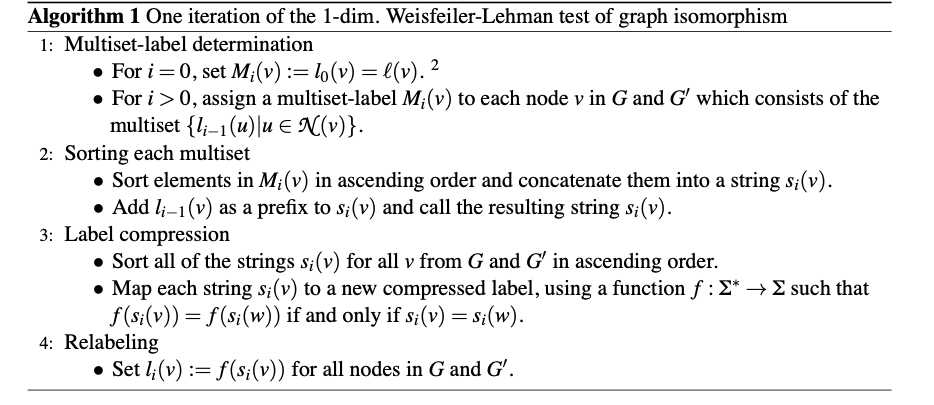
\includegraphics[scale=0.4]{WL algorithm page.png}
	

\end{frame}


\begin{frame}
	\frametitle{Algorithm 1 runtime}
Let $h$ be the number of iterations and $m$ be number of different degree vertices in the two input graphs(??).
	\begin{itemize}
		\item step 1: labelling is $\mathcal{O}(m)$
		\item step 2: sorting is $\mathcal{O}(m)$
		\item Step 3: label compression is $\mathcal{O}(m)$
		\item step 4: relabelling is $\mathcal{O}(m)$
		\item total runtime: $\mathcal{O}(hm)$.
	\end{itemize}

\end{frame}
\begin{frame}
	\frametitle{Another WL GI test}
The following algorithm makes use of a hash function and the WL subtree kernel, which counts original and compressed labels in the input graphs.
	\begin{center}
		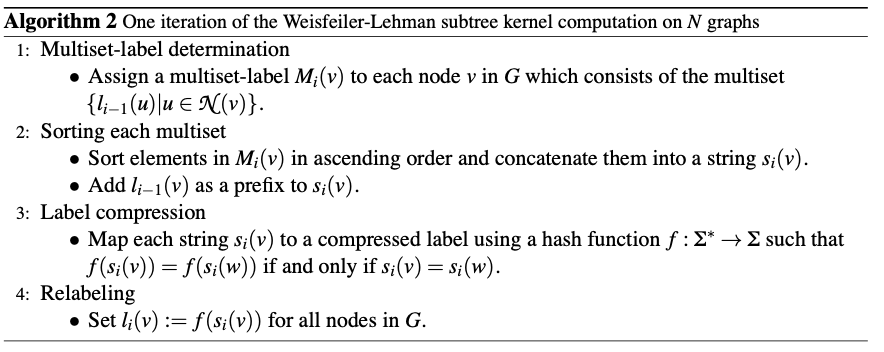
\includegraphics[scale=0.4]{WL alg 2.png}
		\end{center}
	

\end{frame}
\begin{frame}
	\frametitle{Algorithm 2 runtime}
	Algorithm 2 can be run on $N$ graphs, pairwise comparing each graph.
	\begin{block}{Theorem}
		For $N$ graphs, Algorithm 2 with $h$ iterations on all pairs of these graphs can be computed in $\mathcal{O}(Nhm+N^2hn)$.
	\end{block}
Note: $Nhm$ dominates runtime.
 \end{frame}
\begin{frame}
	\frametitle{Algorithm 2 example}
	\begin{center}
	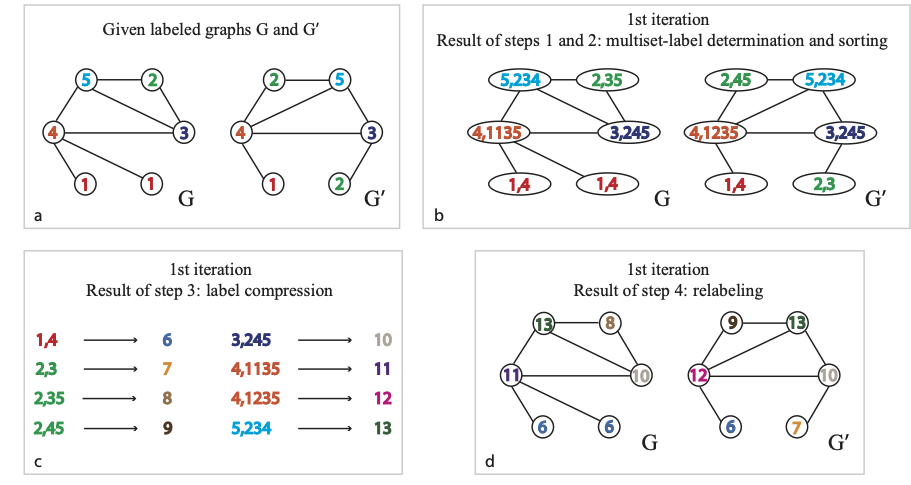
\includegraphics[scale=0.4]{WL example1.png}
	\end{center}

\end{frame}
\begin{frame}
	\frametitle{1-D WL subtree test example}
	\begin{center}
	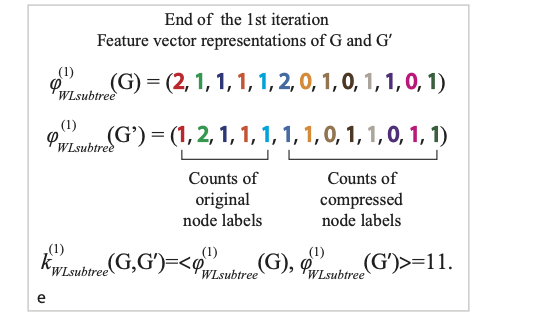
\includegraphics[scale=0.5]{WL example2.png}
	\end{center}

\end{frame}
\begin{frame}
	\frametitle{Algorithm 2 experiments}
	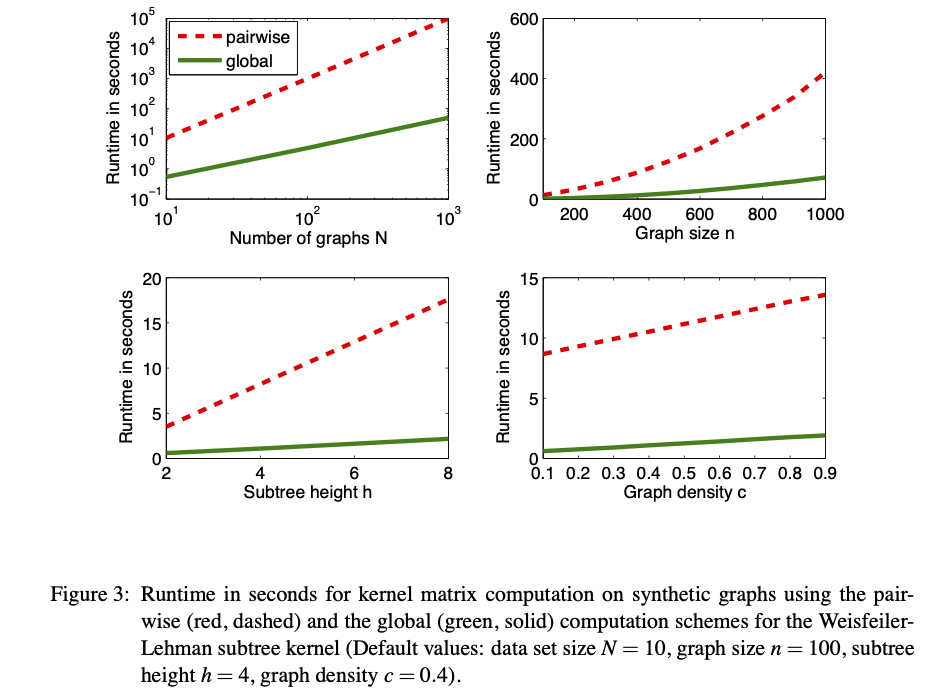
\includegraphics[scale=0.4]{WL results.png}
\end{frame}


\begin{frame}
	\frametitle{How good is 1-D WL in general?}
	It has been shown to be an efficient graph isomorphism test for almost all graphs (Babai, Kucera 1979). There are higher dimensional variants (which I do not understand) that can classify a larger set of graphs. 
\begin{itemize}
	\item 
	\item can be implemented to run in \[\mathcal{O}(n^{k+1}\log n)\] where $k$ is the dimension (k=1 for us) and $n$ is the number of vertices of the input graphs. (Immmerman, Lander 1990)
	\item determining which graphs are classified by any dimension is usually highly nontrivial (see Kiefer (2020))
	\item 1-D WL cannot distinguish regular graphs
	\item other algorithms are better (broader classification abilities and faster) but ideas from WL show up in most of these
\end{itemize}
	

\end{frame}
\begin{frame}
	\frametitle{What's important for GI?}
The powerful solvers are able to say whether or not two graphs are isomorphic or not using canonical labellings and producing the automorphism group of a graph (the set of all isomorphisms from a graph to itself). 
\begin{itemize}
	\item these are complicated 
	\item Babai's isomorphism test is also complicated (he invented new algebra to produce it)
	\item but they both make use of canonical labelling in some way
\end{itemize}
\end{frame}
\begin{frame}
	\frametitle{The practical approach}
Rather than check for isomorphism dirctly, most efficent GI solvers use some form of canonical labelling along with some other fast algorithm.(Mckay 2013). This is called \textit{individualization refinement}.
\begin{block}{individualization refinement}
	input: $G=\{V,E\}$, $G'=\{V',E'\}$\\
	iterate: relabel vertices to produce canonical labelling for $G$\\
	compile: produce automorphism groups of $G$ \\
	output: true or false "$G$ is isomorphic to $G'$" via $G\cong G'$ if and only if $G'\in Aut(G)$
\end{block}
\end{frame}



\begin{frame}
	\frametitle{Applied GI solvers}
Althought the complexity of GI is an open problem, in reality, powerful (open source) software exists for classifying graphs efficently (i.e., they can efficiently proudce the automorphism group containing the set of all graph isomorphisms from a graph to itself). 
\begin{itemize}
	\item Weisfeiler-Leman (color refinement)
	\item nauty
	\item saucy 
	\item bliss
	\item Traces
\end{itemize}
\end{frame}


%\begin{frame}
	%\frametitle{How?}
	%The following outline of an algorithm is tempting.
	%Most efficient software for solving GI does \textit{not} use this approach because it is not suitable for collections of graphs or finding graphs in a database (Mckay 2013).
	%\begin{block}{algorithm}
		%Input: $G=\{V,E\}$, $G'=\${V',E'\}$\\
		%Output: Yes/No there exists graph isomorphism from $G$ to $G'$
	%\end{block}

%\end{frame}

%Neil Immerman and Eric Lander. Describing graphs: a first-order approach to graph canonization. In Alan L. Selman, editor, Complexity theory retro- spective, pages 59–81. Springer, 1990.

%Sandra Kiefer's dissertation "The power and limits of the Weisfeler Leman Algorithm" (2020))

\end{document}